% 1:1 markup translation of paper1_draft.md lines 593-919 (S5, S6).
\section{The tier ladder: three attractor families}

Holding prompt, container and scoring fixed, we varied only the nominal proposer tier across
the three cells that discriminate hardest between prediction and family optimum --- $N = 13$, 21
and 31, each inside a trap zone. The tiers do not merely differ in success rate: they attempt
qualitatively different constructions.

\textbf{The weak tier truncates templates.} The Haiku-tier proposer (Figure~\ref{fig:packings}, left panel) produces uniform grids of radius
$1/(2k)$ truncated to $N$ circles, with corner fillers only when the grid underfills. Across the 45
original bare invocations spanning $N \in \{13, 17, 21, 31, 35, 37, 43\}$, \textbf{35 were geometrically
valid at the primary $10^{-6}$ tolerance (77.8\%), 29 at $10^{-9}$ (64.4\%)} --- recomputed from the ledger,
superseding the figure carried in earlier drafts. At the three discriminating cells 12 of 16 valid samples
landed on the predicted value and the rival was reached twice, both at $N = 21$.

\textbf{The middle tier perturbs and mixes.} The Sonnet-tier arm was preregistered in
\texttt{arm\_s\_preregistration.txt}, disclosing that 5 of 20 samples at $N = 13/21$ had been seen before
registration and that $N = 31$ was fully blind. It was valid 30/30 at $10^{-6}$ and 27/30 (90\%) at
$10^{-9}$ --- so the ``100\%'' leg is tolerance-dependent and both numbers are stated. It was almost
never on-prediction: 0/10, 0/10, 1/10 --- 1/30 pooled against the weak tier's 12/16 at the same
cells. Instead of truncating a uniform grid it perturbs one, with enlarged edge rows, hexagonal
interior rows and two or three distinct radii in the same packing (29/30 multi-radius).

One Sonnet sample at $N = 31$ emitted 27 circles at $r = 1/12$ with 4 corner circles at $r = 1/8$,
summing to 2.7499999991 --- above 2.7485281, the best the family reaches at that $N$. Recomputed
from its stored coordinates, the construction is tangency-tight: minimum pairwise and wall slack
both exactly zero at tolerance zero, the exactly-tangent contacts involving the binary-exact
$r = 1/8$ corner circles while the $r = 1/12$ circles carry small positive slack. It is the only
sample in the study to leave the recipe family upward.

That sample also exposes a scoring defect. At $N = 31$ the family rival (2.7485281) and this
out-of-family value (2.75) differ by $1.47\times10^{-3}$, \emph{inside} the registered $2\times10^{-3}$ window, so the
value classifier counted the escape as a hit on the construction it exceeded. The window was
chosen for the anchor comparison, where the nearest competing value is $\sim$0.15 away, and reused
where it does not fit. Classified by structure instead, Sonnet's rival count at $N = 31$ is 2/10
and pooled 5/30. Every categorical claim in this paper about ``reached the
rival'' or ``left the family'' is made at structure level or at $10^{-6}$, never at $2\times10^{-3}$.

\textbf{The top tier attempts recursive constructions and fails to build them.} The third arm was
invoked through a bare tier alias. We name it \texttt{opus\_alias} throughout and make no claim about
which weights served it: the runtime accepts only the bare alias and exposes no dated
identifier, so the binding is a vendor promise rather than an attestable fact. No version number
appears anywhere in this paper.

That caveat matters: completion-time and token-count anomalies were observed in the unreleased
session transcript for this arm, but the ledger carries no latency or token field, so they
appear in no released artifact and nothing below relies on them.

Under those caveats the arm --- preregistered fully blind in \texttt{arm\_o\_preregistration.txt} --- was
valid in 4 of 30 invocations (13\%) at both tolerances. At every cell it attempted a more
ambitious construction than either other tier: quarter-circle corners at $r = 0.25$ with
Apollonius-style fillers at $N = 13$ (10/10 samples), mixed-radius $4 \times 4$-ish grids at $N = 21$, and a
coarse $3 \times 3$ grid at $r \approx 1/6$ with border strips at $N = 31$ (0/10 valid). Failures are geometric
rather than numerical --- edge strips at $r = 0.03$ placed 0.138 from an $r = 1/6$ grid circle needing
0.197 --- and twice the arm padded to count with zero-radius circles. Valid samples score \emph{below}
the trap they were expected to fall into (1.26--1.41 at $N = 13$ against 1.625). A post-hoc
diagnostic (not preregistered; labeled as such in the repository) finds no evidence of a tolerance
artifact behind the 13\% in this sample: 24 of 26 invalid samples overlap grossly (median maximum overlap
$3.3\times10^{-2}$; radius-shrink repair costs a median 15\% of sum-of-radii), while tolerance-scale
near-misses ($< 2.5\times10^{-5}$) occur instead in 5 of 7 geometry-scored weak-tier failures --- the
exact-tangency grids, not the ambitious constructions.

Two decisions here were made after seeing the data and are recorded as deviations (Table 4).
P-O1, P-O2 and P-O4 are reported \textbf{not evaluable}, on the grounds that a validity collapse of
this size makes an on-prediction tier comparison uninterpretable; P-O3 is trivially satisfied on
4/4 valid samples; the registered disconfirmation --- regression toward the trap --- did not occur.
De-registering three of four predictions in the one arm that disconfirmed is exactly the move
preregistration exists to constrain, which is why it is tabled rather than narrated. And the arm
was initially excluded from the ladder, then included once its results were known; we follow the
later decision and report the ladder both ways (Table~\ref{tab:ladder}) --- with the arm 83\% $\rightarrow$ 100\% $\rightarrow$ 13\% on matched cells (78\% over all seven weak-tier cells), without it
83\% $\rightarrow$ 100\% plus the qualitative shift from truncation to perturbed multi-radius hybrids, which
is already the publishable contrast.

\begin{table}[t]
\centering
\caption{Three-attractor ladder. Valid columns count samples passing containment and non-overlap at the $10^{-6}$ and $10^{-9}$ tolerances; On-pred and Rival count valid samples landing on the predicted value and on the rival argmax.}
\label{tab:ladder}
\footnotesize
\setlength{\tabcolsep}{4pt}
\begin{tabular}{@{}p{1.7cm}p{1.2cm}cp{2.2cm}p{1.0cm}p{1.0cm}p{1.5cm}cp{2.0cm}@{}}
\toprule
Tier & Cells & $n$ & Attempted family & Valid $10^{-6}$ & Valid $10^{-9}$ & On-pred & Rival & Failure mode \\
\midrule
haiku (bare) & 13, 17, 21, 31, 35, 37, 43 & 45 & uniform grid, truncated; fillers when underfull & 35 (78\%) & 29 (64\%) & 12/16 (3 matched cells) & 2 & overlap 6, outside 1, parse 3 \\
haiku, matched cells & 13, 21, 31 & 60 & as above & 50 (83\%) & --- & 35/50 & 2 & overlap 5, outside 2, parse 3 \\
sonnet & 13, 21, 31 & 30 & perturbed grid, hexagonal rows, 2--3 radii & 30 (100\%) & 27 (90\%) & 1/30 & 5 (structure) & none \\
\texttt{opus\_alias} $\ddagger$ & 13, 21, 31 & 30 & quarter-circle corners, Apollonius fillers, coarse grid + border strips & 4 (13\%) & 4 (13\%) & 0/4 & 0 & overlap 24, nonpositive radius 2 \\
\bottomrule
\end{tabular}
\end{table}

$\ddagger$ Addressed through a bare serving alias; the alias-to-weights binding is not attestable, and
this row is not a statement about any released model version. Tier denominators are not matched
(the weak tier spans seven $N$ against three), which is why the matched-cell row is given
separately, and it is the matched comparison (83\% $\rightarrow$ 100\% $\rightarrow$ 13\%) that should be quoted across
tiers. Sources: \texttt{arm\_f\_candidates\_v2.jsonl}, the three preregistration files.

\begin{figure}[t]
\centering
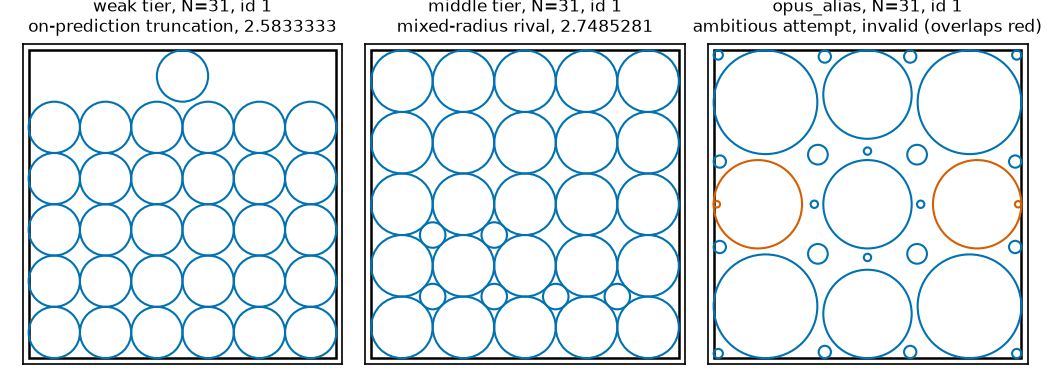
\includegraphics[width=\linewidth]{fig2_packings.png}
\caption{\emph{Three attractor families at a single cell, $N = 31$.} One representative packing
per tier, ledger sample id in each panel title (weak tier \texttt{bare} id 1, on-prediction truncation
2.5833333; middle tier \texttt{sonnet\_bare} id 1, mixed-radius rival 2.7485281; \texttt{opus\_alias} id 1,
invalid, with only the offending circles highlighted). Source: \texttt{arm\_f\_candidates\_v2.jsonl} via
\texttt{fig\_scripts.py}, deterministic (the exemplar rows' geometry is byte-identical in v1; v2 differs
only in provenance metadata).}
\label{fig:packings}
\end{figure}

``Monotone'' applies to one axis only: ambition rises monotonically ---
truncated template, perturbed hybrid, recursive gasket --- while validity rises then collapses.
``Ambition'' is measurable, not merely a qualitative read: a post-hoc diagnostic (disclosed;
\texttt{diagnostics\_ambition.py}, all samples with emitted geometry, invalid included) gives median
distinct radii per sample 1 $\rightarrow$ 2 $\rightarrow$ 3 (means 1.33 $\rightarrow$ 2.40 $\rightarrow$ 3.37) and median off-lattice center
fraction 0.08 $\rightarrow$ 0.43 $\rightarrow$ 0.95 across the three tiers --- monotone on both operationalizations. At
the canonical and plausibly contaminated cell $N = 26$ all tiers converge on the same 2.5414
attractor; they diverge only at withheld trap cells. The branch rule of \S2 is therefore a
weak-tier regularity --- cross-vendor under two instruments (a registered pooled bar under
GM3's, carried by its non-discriminating cells, \S3.6; 61--67\% of valid outputs in two further
vendors under arm V's, \S3.6), family-bounded in both directions (absent in gemma-4-31b at
the same floor, escaped \emph{upward} to the family rival by gemma-4-26b, \S3.6), cell-level modes
confirmed in one lineage --- and
this is a \textbf{boundary condition on the main result}, not an independent
second finding. It also cuts against \S1's framing: the discovery systems cited there run
frontier or mid-tier proposers, so the tier at which our regularity holds is the tier they do not use,
while the tier closest to what they use escapes the trap in our own data.

\section{Elicitation and faithfulness}

This section is explicitly secondary material and the result leans negative: the registered
validity prediction fails, the concentration effect survives only as a fragile directional
finding, and the faithfulness audit checks description against artifact, not against process.

\subsection{Design and bundling disclosure}

A ten-versus-ten pilot at $N = 21$ compared the bare prompt against a variant asking the proposer to
name its construction on a leading \texttt{METHOD:} line: validity rose from 7/10 to 10/10 and the
higher-scoring rival disappeared, from 2 of 7 valid bare samples to 0 of 10 trace samples. Before
any scaled sample was drawn we registered four predictions and an explicit falsifier in
\texttt{arm\_t\_preregistration.txt} (sha256 \texttt{ab7900a8\ldots}), disclosing that the pilot's trace prompt had
drifted from the bare template beyond the method line --- it omitted the \texttt{[0,1]x[0,1]} tokens and
reworded the output-format line --- so the pilot's intervention was method-line-plus-rewording,
bundled. Pilot samples are never pooled with \texttt{trace\_v2}.

The scaled prompt, \texttt{trace\_v2}, is itself a \textbf{bundled prompt-format-and-trace-request}
intervention, though a near-minimal diff: one inserted \texttt{METHOD:} line, plus \texttt{"After the METHOD
line, "} prepended to the output line and \texttt{"no other text"} changed to \texttt{"no other text after the
list"}. That second change is not cosmetic --- \S6.2 shows it doing measurable work --- so the measured
effect is \emph{method-line-plus-output-line-rewording}, not the method line alone: a weaker version of
the confound for which the pilot was discarded, held to the same standard.

The scaled arm ran 100 new invocations, bringing both arms to 20 per cell at $N \in \{13, 21, 31\}$ and
the corpus to 215 logged square invocations (85 bare = 45 original + 40 new; 70 trace = 10 pilot +
60 trace\_v2; 30 sonnet; 30 \texttt{opus\_alias}), plus 16 rectangle invocations, 231 total before the
extension arms; arm M (\S3.4) added 57 sampled
weak-tier invocations (60 launched), bringing the study corpus to 288, and
arms MU and CH (\S3.5) added 180 more (180 launched, none lost), and the code-channel arms
CC, CC2 and CCS (\S3.7) added 135 more (135 launched, none lost), bringing the
unconditioned-and-elicitation corpus to 603, and the held-out-$N$ probe CN (\S3.8) 75 more, to 678; the cross-vendor chain is scored under its own
registrations and adds 420 GM-chain invocations (\S3.6, \S8) and 877 arm-V attempt rows over
325 registered invocation slots (\S3.6). One disclosure: \textbf{20 of the 60 bare samples are pre-existing arm-F
rows} ($N = 13$ ids 1--5, $N = 21$ ids 1--10, $N = 31$ ids 1--5) whose results were known when P-T1--P-T3
were written; only trace\_v2 is fully fresh (\S6.4). Scoring used \texttt{arm\_f\_repro.py} unchanged with
the registered $2\times10^{-3}$ window; the Fisher exact test comes from the hypergeometric tail in
\texttt{arm\_t\_analysis.py}, checked against a reference.

\subsection{Registered outcomes}

Preregistered criteria are evaluated exactly as registered, and unregistered alpha thresholds are
applied nowhere.

\textbf{P-T1, validity: NOT confirmed.} P-T1 is the one prediction that registered an alpha (``validity
$\ge$ bare at EACH $N$, and pooled one-sided Fisher $p < 0.05$''). Direction held at all three cells, but
the pooled test gives $p = 0.30$: 53/60 (88\%) trace\_v2 against 50/60 (83\%) bare, a difference whose
detection needs several hundred samples per arm at 80\% power --- a failure to detect, not a
demonstration of no effect. The direction that did hold is not geometric: bare
had \textbf{3 parse failures and 7 geometric failures}, trace\_v2 \textbf{0 parse and 7 geometric}, so among
parsed samples geometric validity is 50/57 (87.7\%) versus 53/60 (88.3\%). The P-T1 direction is
format compliance, exactly what the reworded output-format line manipulates; validity is reported
split by cause from here on.

\textbf{P-T2, rival suppression: CONFIRMED as registered} (directional, no alpha): 1 of 53 valid
trace\_v2 against 2 of 50 valid bare. Counts this near zero carry no inferential weight and we
claim none (Fisher $p = 0.48$, carrying no decision). One trace\_v2 sample at $N = 31$ hit the rival
2.7485281 to within $3.6\times10^{-8}$ --- the first weak-tier rival hit at $N = 31$ in any arm, and formerly
one of the scorer's mismatches (\S6.5).

\textbf{P-T3, anchor concentration: met as registered (directional), inferentially fragile.} Among
valid samples, 46 of 53 trace\_v2 (87\%) landed on the registered prediction against 35 of 50 (70\%)
bare. The $p$-value it never carried is 0.0325, one-sided uncorrected (\S6.4).

\textbf{P-T4, faithfulness: confirmed under a corrected scorer.} The registered scorer gives 38 of 41
scoreable claims matching (93\%) against a 90\% threshold; blind hand-adjudication under a rubric
frozen before rescoring gives 54 of 56 (96.4\%). \S6.5 reports both.

\begin{table}[t]
\centering
\caption{Paired trace grid (scaled arm only).}
\label{tab:tracegrid}
\begin{tabular}{@{}llcccc@{}}
\toprule
$N$ & Arm & $n$ & Valid (parse / geom. fail) & On-pred / valid & Rival \\
\midrule
13 & bare & 20 & 18 (0 / 2) & 10 (56\%) & 0 \\
13 & trace\_v2 & 20 & 18 (0 / 2) & 16 (89\%) & 0 \\
21 & bare & 20 & 15 (1 / 4) & 12 (80\%) & 2 \\
21 & trace\_v2 & 20 & 18 (0 / 2) & 16 (89\%) & 0 \\
31 & bare & 20 & 17 (2 / 1) & 13 (76\%) & 0 \\
31 & trace\_v2 & 20 & 17 (0 / 3) & 14 (82\%) & 1 \\
\textbf{pooled} & bare & 60 & 50 (3 / 7) & 35 (70\%) & 2 \\
\textbf{pooled} & trace\_v2 & 60 & 53 (0 / 7) & 46 (87\%) & 1 \\
\bottomrule
\end{tabular}
\end{table}

Per-cell one-sided Fisher on on-prediction (Figure~\ref{fig:armT}): $N = 13$ $p = 0.030$; $N = 21$ $p = 0.41$; $N = 31$ $p = 0.50$.
Pooled $p = 0.0325$; Holm threshold over the registered family ($m = 3$ tested with $p$-values) is
0.0167. The pilot (10 invocations at $N = 21$, 10/10 valid, 9/10 on-prediction) is reported
separately and never summed into any total. Regenerated by \texttt{arm\_t\_analysis.py} over
\texttt{arm\_f\_candidates\_v2.jsonl}.

\begin{figure}[t]
\centering
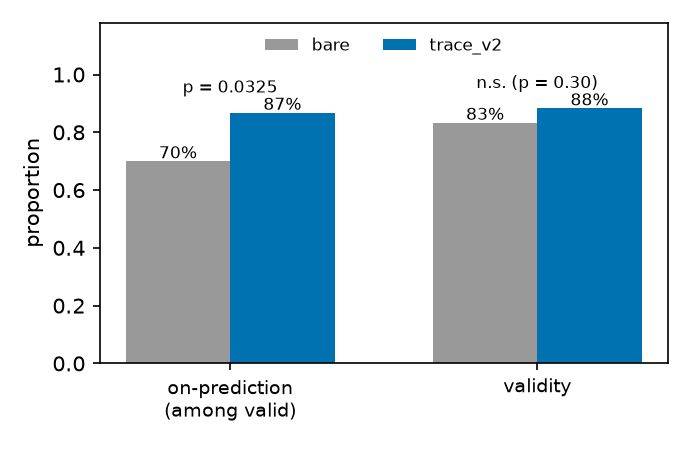
\includegraphics[width=\linewidth]{fig3_armT.png}
\caption{\emph{Bare versus \texttt{trace\_v2}, by cell and pooled.} Caption caveat: the bars pool the
bare arm's two collection waves, which \S6.4 shows drift materially, so the pooled bare bar is a
mixture; the same-wave comparison in \S6.4 is the wave-controlled picture.}
\label{fig:armT}
\end{figure}

\subsection{The registered falsifier, both readings}

The registered falsifier reads: \emph{``if trace\_v2 validity \texttt{<=} bare at 2+ of 3 N, the pilot effect
was the bundled rewording, not the method-line request --- reported as such, not reframed.''}
Observed validity: $N = 13$, 18/20 both arms --- \textbf{tie}; $N = 21$, trace\_v2 18/20 against bare 15/20 ---
trace higher; $N = 31$, 17/20 both arms --- \textbf{tie}. A tie satisfies \texttt{<=}, so under the registered
wording the falsifier is \textbf{triggered at 2 of 3 $N$}, and we report it as triggered; the code
instead evaluated direction as \texttt{t\_rate >= b\_rate}, strict \texttt{<}, under which it fires at 0 of 3
cells. That convention appears nowhere in
the preregistration, was chosen at analysis time, and read the same tie favorably twice --- as
``direction held'' for P-T1 and as ``not a falsifier cell'' here.

We name the failure mode \textbf{operationalization drift between preregistration text and analysis
code}: registered prose leaves boundary behavior --- ties, inclusive versus exclusive bounds,
rounding --- implicit, and the scorer must choose after the data exist; the preregistration
literature (\S7) discusses what is locked, not this tie-handling layer. Remedies, free before
sampling and impossible afterward: register the comparison as executable code, or state the tie
convention in the registration text. \texttt{arm\_t\_analysis.py} now prints both readings and names the
registered tie-inclusive one authoritative. Under that reading \textbf{the pilot's validity effect is
attributed to the bundled rewording, not to the method-line request}, as the falsifier clause
instructed; the \S6.2 parse-versus-geometric split points the same way, and P-T1 fails under both
readings regardless.

\subsection{Limits of P-T3: what the concentration result will and will not carry}

P-T3 met its registered directional criterion. It is not a flagship result.

\emph{No registered alpha.} P-T3 registered direction only; the $p$-value is a post-hoc addition.

\emph{Multiplicity.} Of four registered predictions, three are reported with $p$-values. Holm sets the
first threshold at $0.05/3 = 0.0167$; $p = 0.0325$ fails it, as it fails Bonferroni at any $m \ge 2$ and
Benjamini--Hochberg FDR at $q = 0.05$. Two-sided Fisher is $p = 0.0537$. P-T3 is nominally significant
uncorrected and is not under family-wise error control.

\emph{Concentration in one cell.} Per-cell tests give $p = 0.030$, 0.41, 0.50 (Table 3); the pooled
17-point gap is a 33-point gap at $N = 13$ averaged with 9- and 6-point gaps elsewhere, driven by a
\emph{low bare rate at $N = 13$} ($10/18 = 56\%$) rather than a high trace rate --- the trace rate there (89\%)
equals that at $N = 21$. Dropping $N = 13$, the comparison is 30/35 vs 25/32, $p = 0.31$.

\emph{Wave confound.} The bare arm mixes two collection waves; trace\_v2 is one. Splitting bare on the
registered id boundary, with no intervention applied to either half, on-prediction is: $N = 13$, 3/4
old wave vs 7/14 new; $N = 21$, 4/7 vs 8/8; $N = 31$, 5/5 vs 8/12 --- the control arm's own
between-wave drift is comparable to the effect attributed to the manipulation. (An earlier
draft printed 2/4 vs 10/11 at $N = 21$ and a 25/37 pooled figure --- arithmetically impossible
against \S6.1's id boundary; corrected here from the ledger.) Restricting to one
wave, new-wave bare is 23/34 (68\%) against trace\_v2's 46/53 (87\%), but \textbf{this stratified
comparison is post hoc, not preregistered, no confirmatory weight} --- a diagnosis, not a rescue:
wave is a confound \emph{in the registered analysis}, which cannot separate it from the manipulation.
The design fix, interleaved collection in one session, was not run.

\emph{What we therefore claim.} A minimal method-naming request does not make the proposer better at
geometry and does not measurably change which rare constructions it reaches; in the registered
direction it concentrates output onto the anchor, but that concentration fails correction, is
carried by one cell, is confounded with collection wave, and is bundled with an output-format
rewording that demonstrably affects parse compliance. Studies collecting process descriptors \emph{by
asking for them}, including descriptor-driven quality-diversity pipelines where the descriptor is
a requested self-report, should treat this as a reason to check, not a coefficient to apply. The
pilot also showed a \emph{third} effect in the P-T3 direction at the same cell (trace 9/10
on-prediction against bare $N = 21$ at 4/7, one-sided $p = 0.16$), so P-T3 replicated a pilot signal
rather than testing a blind prediction --- a different status, and the prereg's pilot disclosure
covered the prompt drift only.

\subsection{Faithfulness with ground truth}

Claim and artifact sit in the same completion and the artifact is fully determined, so a method
line is checkable against the emitted coordinates. \texttt{arm\_f\_repro.trace\_faithfulness()} matches
numeric dimensions from the method line against the emitted layout signature, returning 38 of 41
scoreable claims matching (93\%) against the registered 90\% threshold. Its 12 exclusions are regex
coverage gaps, not claims without numeric content: \texttt{DIMS\_RE} matched only the
literal \texttt{NxN} form and \texttt{ROWSCOLS\_RE} required rows before columns, so these fell through despite
carrying explicit checkable dimensions --- ``Regular 3 by 4 grid with one additional circle in row
4''; ``3 complete rows of 4 circles and 1 centered circle in the top row''; ``rectangular grid 4-4-4-1
with uniform radius 1/8''; ``Four-row grid with 4 circles in the first row and 3 in each of the
remaining''; ``Rectangular grid arrangement with 5 columns and 4 rows, plus one additional circle on
top edge''; ``Square grid 5 columns 4 rows with 1 additional circle at top''; ``Rectangular grid six
columns by six rows radius one-twelfth with five circles removed''; ``Regular 5-column by 6-row grid
plus one additional circle in the right margin''; ``Rectangular grid packing with five columns and
six rows plus one additional circle''. Three further exclusions --- ``Uniform horizontal strips with
tight row spacing'', ``Regular rectangular grid packing with corner circle'', ``Equal-radius
rectangular grid with 4 rows stacked vertically'' --- are closer to genuinely unscoreable. The
excluded set is enriched for non-canonical phrasings, where a mismatch is a priori \emph{more} likely,
so the exclusion was not conservative in a known direction; worst case, had all 12 been
unfaithful, the rate would have been $38/53 = 72\%$.

\textbf{Blind rescore under a frozen rubric.} The rubric (\texttt{p7\_faithfulness\_rubric.md}) --- checkable
assertions in any surface form, plus match rules including a base-grid convention for ``grid plus
additions'' claims and a truncation convention for ``with k removed'' claims --- was committed to git
as \texttt{e181d2a} at 03:56:56 on 2026-08-01, \textbf{before} any rescoring run, so the freeze is checkable,
and it pre-committed the reporting rule: below 90\%, P-T4 reported not confirmed, full stop, no
consolation framing. Scoring was blind --- claim text and circles only, no predicted or rival
values, no running tally, no threshold and no sight of the existing 38/41 result --- with tallying
afterward; all 60 labels are released verbatim in \texttt{p7\_blind\_labels.json}.

\textbf{Result.} Over all 60 trace\_v2 rows: \textbf{54 MATCH, 2 MISMATCH, 4 UNSCOREABLE} --- a corrected rate
of \textbf{54/56 = 96.4\%} of scoreable claims, Wilson 95\% CI $[88\%, 99\%]$, passed, and on 56 scoreable
claims rather than 41. The CI's lower bound sits just below the registered threshold, so ``clears
90\%'' is a statement about the point estimate at this $n$. The two mismatches share a form: row 11
claims ``alternating rows of 4 and 3 circles'' over observed row sizes 4,3,3,3, row 33 claims ``5
rows alternating between 5 and 4 circles'' over observed 5,4,4,4,4 --- both \emph{mis-descriptions of
alternation}, a repeating pattern named and built for the first period only. The original scorer's
three mismatches were three different claim forms, not one; the filler-adds-
rows mechanism the original scorer described was real, and the rubric's base-grid convention handles it, so
all three score MATCH under hand adjudication.

\textbf{Scope, three ways.} The blind pass covers \emph{invalid} rows too: the original 93\% conditioned on
completions that produced a correct packing --- the wrong conditioning, since a method line attached
to an overlapping layout is where description and artifact are likeliest to diverge --- while the
blind pass scored all 60 rows including the 7 invalid ones, 4 of the 60 unscoreable. Second, the
check verifies the description against the \emph{artifact}, not the process: the non-claim guard
applies in full, and for a model already emitting grids, ``$5 \times 5$ grid'' matching a $5 \times 5$ grid is closer
to a self-consistency check than to the causal question the chain-of-thought literature asks (\S7).
Third, the audit is confounded with the elicitation arm, computed on the arm \S6.2 shows
concentrates 87\% of valid outputs onto one template, where correct description is close to free;
faithfulness is informative precisely on off-template outputs, such as the pilot's
triangular-hexagonal 6+5+4+3+2+1 sample, described exactly while summing to 1.75. The split by on-
versus off-prediction is not run here (\S9, stopping rule). What survives is narrow: in a domain
where claims are checkable, the method lines this proposer emits are, at 54 of 56 scoreable
claims, true of the object it produced --- and both failures are a model describing a pattern it
started and did not finish.
